\documentclass[12pt,a4paper]{report}

% Layout follows the IIIT Kottayam BTP report template (12 pt, 1.5 spacing, title page,
% declaration, certificate). The template's play/pstcol/xy packages are not needed here.
\usepackage[a4paper,left=1.25in,right=1in,top=1in,bottom=1in]{geometry}
\usepackage{amsmath,amssymb,amsthm,mathrsfs,setspace}
\usepackage{graphicx,booktabs,array,multirow,caption,subcaption,xcolor,rotating}
\usepackage{cite}          % sorts and compresses the numbers inside one bracket: [3, 12], [3–5]
\usepackage[nottoc]{tocbibind}
\usepackage{tikz}
\usetikzlibrary{arrows.meta,positioning,shapes.geometric,fit,calc}
\usepackage{microtype}
\usepackage[hidelinks]{hyperref}
\emergencystretch=2em
\usepackage{enumitem}
\setlist{itemsep=2pt,topsep=4pt}
\renewcommand{\chaptermark}[1]{\markboth{#1}{}}
\renewcommand{\sectionmark}[1]{\markright{\thesection\ #1}}

\theoremstyle{plain}
\newtheorem{theorem}{Theorem}[section]
\newtheorem{lemma}[theorem]{Lemma}
\newtheorem{proposition}[theorem]{Proposition}
\theoremstyle{definition}
\newtheorem{definition}[theorem]{Definition}
\theoremstyle{remark}
\newtheorem{remark}[theorem]{Remark}

% 1.5 spacing for the text; tables, figures and their captions single-spaced
\setstretch{1.5}
\usepackage{etoolbox}
\AtBeginEnvironment{table}{\setstretch{1.0}}
\AtBeginEnvironment{figure}{\setstretch{1.0}}
% less white space above chapter titles; the contents list chapters and sections
\makeatletter
\patchcmd{\@makechapterhead}{\vspace*{50\p@}}{\vspace*{10\p@}}{}{}
\patchcmd{\@makeschapterhead}{\vspace*{50\p@}}{\vspace*{10\p@}}{}{}
\patchcmd{\@makechapterhead}{\vskip 40\p@}{\vskip 25\p@}{}{}
\patchcmd{\@makeschapterhead}{\vskip 40\p@}{\vskip 25\p@}{}{}
\makeatother
\setcounter{tocdepth}{2}

% ---------------------------------------------------------------- project data
\newcommand{\projecttitle}{Privacy-Preserving Authentication and Authorization for VANETs Using Blockchain and Zero-Knowledge Proofs}
\newcommand{\reportdate}{November 2026}
\newcommand{\guide}{Dr. Deepak Jose}

% Measured numbers come from experiments/thesis_data.py (generated/numbers.tex):
% \R{key}{metric}, e.g. \R{cmp/v3-fast}{ticket_ms_mean}. A missing one prints a bold ??.
\makeatletter
\newcommand{\R}[2]{\ifcsname r@#1@#2\endcsname\csname r@#1@#2\endcsname\else\textbf{??}\fi}
\makeatother
\InputIfFileExists{generated/numbers.tex}{}{}
% a figure from generated/fig, or a visible placeholder while its sweep is pending
\newcommand{\genfig}[2][0.8\textwidth]{%
  \noindent\IfFileExists{generated/fig/#2.pdf}{\includegraphics[width=#1]{generated/fig/#2.pdf}}%
  {\fbox{\parbox[c][4cm][c]{\dimexpr#1-2\fboxsep-2\fboxrule}{\centering\small Figure pending:
  \texttt{\detokenize{#2}}\\(make evaluate-all, then thesis\_data.py)}}}}
\newcommand{\gentab}[1]{\InputIfFileExists{generated/#1.tex}{}{\fbox{Table pending: #1}}}

\begin{document}

% --------------- Title page -----------------------
\pagenumbering{Alph}
\begin{titlepage}
\enlargethispage{2cm}
\begin{center}
\vspace*{-1cm}
\textbf{\Large PRIVACY-PRESERVING AUTHENTICATION AND AUTHORIZATION FOR VANETS USING BLOCKCHAIN AND ZERO-KNOWLEDGE PROOFS}\\[10pt]
\vspace*{1.2cm}
A Project Report Submitted \\
in Partial Fulfilment of the Requirements \\
for the Degree of \\
\vspace{4.10mm}
{\Large \bf Bachelor of Technology} \\
in \\
{\large \bf Computer Science and Engineering}\\
with Specialization in\\
{\large \bf Cyber Security} \\
\vspace{3.85mm}
{\em by} \\ \vspace{2.15mm}
{\large \bf Ben Savio - 2023BCY0009}\\
{\large \bf Harsh Kumar Gour - 2023BCY0010}\\
{\large \bf Byreddy Varshith Reddy - 2023BCY0063}\\
{\large \bf Andela Harsha Vardhan - 2023BCY0024}\\
\vspace{4mm}

\includegraphics[width=5cm, height=2.85cm]{logo2.jpg}\\
\vspace*{0.1cm}
{\em\large to}\\
{\bf \mbox{DEPARTMENT OF CSE-CYBER SECURITY}}\\
{\bf \mbox{INDIAN INSTITUTE OF INFORMATION TECHNOLOGY}}\\
{\bf KOTTAYAM-686635, INDIA}\\
{\it \reportdate}
\end{center}
\end{titlepage}

\clearpage
% --------------- Declaration -----------------------
\pagenumbering{roman}\setcounter{page}{2}
\begin{center}{\large\bf DECLARATION}\end{center}

\sloppy\noindent We, \textbf{Ben Savio} (\textbf{Roll No: 2023BCY0009}), \textbf{Harsh Kumar Gour}
(\textbf{Roll No: 2023BCY0010}), \textbf{Byreddy Varshith Reddy} (\textbf{Roll No: 2023BCY0063})
and \textbf{Andela Harsha Vardhan} (\textbf{Roll No: 2023BCY0024}), hereby declare that this report
entitled \textbf{``\projecttitle''} submitted to Indian Institute of Information Technology Kottayam
towards partial requirement of {\bf Bachelor of Technology} in \textbf{Computer Science and
Engineering} with specialization in \textbf{Cyber Security} is an original work carried out by us
under the supervision of \textbf{\guide} and has not formed the basis for the award of any degree or
diploma, in this or any other institution or university. We have sincerely tried to uphold the
academic ethics and honesty. Whenever an external information or statement or result is used then,
that have been duly acknowledged and cited.

\vspace{2.5cm}
\noindent Kottayam-686635 \hfill \textbf{Ben Savio}\\
\noindent \reportdate \hfill \textbf{Harsh Kumar Gour}\\
\mbox{}\hfill \textbf{Byreddy Varshith Reddy}\\
\mbox{}\hfill \textbf{Andela Harsha Vardhan}
\clearpage

% --------------- Certificate -----------------------
\begin{center}{\large\bf CERTIFICATE}\end{center}

\sloppy\noindent This is to certify that the work contained in this project report entitled
\textbf{``\projecttitle''} submitted by \textbf{Ben Savio} (\textbf{Roll No: 2023BCY0009}),
\textbf{Harsh Kumar Gour} (\textbf{Roll No: 2023BCY0010}), \textbf{Byreddy Varshith Reddy}
(\textbf{Roll No: 2023BCY0063}) and \textbf{Andela Harsha Vardhan} (\textbf{Roll No: 2023BCY0024})
to the Indian Institute of Information Technology Kottayam towards partial requirement of
{\bf Bachelor of Technology} in \textbf{Computer Science and Engineering} with specialization in
\textbf{Cyber Security} has been carried out by them under my supervision and that it has not been
submitted elsewhere for the award of any degree.

\vspace{4cm}
\noindent Kottayam-686635 \hfill (\guide)\\
\noindent \reportdate \hfill Project Supervisor
\clearpage

% --------------- Acknowledgement -----------------------
\begin{center}{\large\bf ACKNOWLEDGEMENT}\end{center}
\addcontentsline{toc}{chapter}{Acknowledgement}

We express our sincere gratitude to our project guide, \guide, for his guidance, encouragement
and valuable suggestions throughout this work; his feedback at the Phase~I review shaped the
direction of the implementation and its evaluation. We thank the Department of CSE-Cyber Security,
Indian Institute of Information Technology Kottayam, for the facilities and the academic environment
that made this project possible, and the faculty and staff of the department for their support.
We also acknowledge the authors and maintainers of the open tools and datasets this work builds on:
ns-3, SUMO, the Luxembourg SUMO Traffic (LuST) scenario, the VeReMi Extension dataset and
Hyperledger Fabric.

\vspace{2cm}
\noindent\hfill Ben Savio \quad Harsh Kumar Gour \quad Byreddy Varshith Reddy \quad Andela Harsha Vardhan
\clearpage

% --------------- Abstract -----------------------
\begin{center}{\Large\bf ABSTRACT}\end{center}
\addcontentsline{toc}{chapter}{Abstract}
Vehicles in a vehicular ad hoc network (VANET) broadcast safety messages about ten times a second.
These messages must be authentic, must not let an observer track a vehicle, and must stay small
enough for a shared radio channel. Existing schemes trade these goals against each other.

This project designs, implements and evaluates a scheme that combines them. A trusted authority
registers each vehicle's pseudonyms in a Merkle tree and publishes only its root on a permissioned
Hyperledger Fabric ledger. A vehicle authenticates to a roadside unit (RSU) with a Schnorr
zero-knowledge proof of membership bound to the RSU's fresh nonce, the requested service and its
vehicle class, and receives a short-lived ticket that it uses to sign its safety messages and to
hand over between RSUs. Smart-contract policies decide which vehicle classes may use which service.
RSUs run a misbehaviour detector, report suspicious pseudonyms to the ledger, where two reports
revoke a pseudonym, and a threshold of RSU organizations can jointly unmask a revoked vehicle, which
then loses all of its pseudonyms. The work further adds TESLA broadcast authentication, implicit
certificates, dead-reckoning message triggering, revocation filters and emergency vehicles.

The system runs on ns-3 (IEEE 802.11p) with SUMO mobility on a grid and on real Luxembourg traffic
(LuST), with measured cryptographic costs, against an IEEE 1609.2-style certificate baseline and a
central authority. At \R{cmp}{vehicles} vehicles on the grid, a zero-knowledge login takes
\R{cmp/v3-fast}{ticket_ms_mean}\,ms, as fast as presenting a certificate
(\R{cmp/ECDSA-PKI}{ticket_ms_mean}\,ms) and far faster than a central authority
(\R{cmp/Central-TA}{ticket_ms_mean}\,ms). The scheme puts \R{cmp/derived}{safety_factor} times less
safety traffic on the channel than certificate-signed messages, lowers the channel busy ratio from
\R{cmp/ECDSA-PKI}{cbr_rsu_mean} to \R{cmp/v3-fast}{cbr_rsu_mean}, and lets vehicles reject messages
from revoked senders (\R{cmp/v3-fast}{v2v_revoked_accepted_ratio} still accepted), while every
attacker is caught and no honest vehicle is revoked. Its login costs about as much computation as
BPA and far less than ZAMA and B-TSCA, priced with the same unit costs. On the
VeReMi Extension dataset the detector reaches an F1 score of \R{veremi}{hgb_window_f1}, up from
\R{veremi}{rules_f1} for plausibility rules alone. A Fabric~3.1.5 benchmark compares Raft and
SmartBFT ordering for the ledger operations.

\vspace{0.5em}
\noindent\textbf{Keywords:} VANET, zero-knowledge proof, permissioned blockchain, Hyperledger Fabric,
conditional privacy, revocation, misbehaviour detection, ns-3, SUMO.

\clearpage

\fussy
% the lists are single-spaced, and the lists of figures and tables share pages
\begingroup\setstretch{1.0}
\tableofcontents
\clearpage
\listoffigures
\let\clearpage\relax
\listoftables
\endgroup
\chapter*{List of Abbreviations}
\addcontentsline{toc}{chapter}{List of Abbreviations}
\begin{tabular}{@{}p{3cm}p{11cm}@{}}
BBS & Boneh--Boyen--Shacham signatures (anonymous credentials)\\
BFT & Byzantine fault tolerance\\
BSM & Basic Safety Message (``here I am'' broadcast, SAE J2735)\\
CBR & Channel busy ratio\\
CI & Confidence interval\\
DR & Dead reckoning\\
ECDSA & Elliptic Curve Digital Signature Algorithm\\
ECQV & Elliptic Curve Qu--Vanstone implicit certificates\\
F1 & Harmonic mean of precision and recall\\
ITS & Intelligent Transportation Systems\\
LuST & Luxembourg SUMO Traffic scenario\\
MSP & Membership Service Provider (Hyperledger Fabric)\\
OBU & On-board unit\\
PDR & Packet delivery ratio\\
PKI & Public-key infrastructure\\
RSU & Roadside unit\\
SCMS & Security Credential Management System\\
SUMO & Simulation of Urban MObility\\
TA & Trusted authority\\
TESLA & Timed Efficient Stream Loss-tolerant Authentication\\
V2I / V2V & Vehicle-to-infrastructure / vehicle-to-vehicle\\
VANET & Vehicular ad hoc network\\
ZKP & Zero-knowledge proof\\
\end{tabular}


\clearpage
\pagenumbering{arabic}\setcounter{page}{1}

\chapter{Introduction}\label{ch:intro}

Road vehicles are becoming networked computers. Through dedicated short-range radio, a vehicle can
tell the vehicles around it where it is, how fast it is going and that it is braking, long before a
driver could see the danger. Intelligent Transportation Systems (ITS) build collision warnings,
cooperative intersection management and emergency-vehicle preemption on these messages. Their value
depends on one question that the radio alone cannot answer: can the message be trusted? This report
describes a system that answers it without giving up the privacy of the people in the vehicles, and
measures what that costs on a realistic network.

\section{Vehicular Ad Hoc Networks}

A vehicular ad hoc network (VANET) consists of three kinds of participants:
\begin{itemize}
  \item \textbf{On-board units (OBUs):} the radio computers in vehicles. They broadcast a
  \emph{Basic Safety Message} (BSM)~\cite{saej2735}, also called a cooperative awareness message
  in Europe~\cite{etsi302637}, about ten times per second, with position, speed and heading.
  \item \textbf{Roadside units (RSUs):} fixed radios at junctions with a wired backbone connection.
  They authenticate vehicles, relay information and act as the network's local infrastructure.
  \item \textbf{A trusted authority (TA):} for example a transport department, which registers
  vehicles. It is not on the communication path during normal operation.
\end{itemize}
Vehicles talk to each other (V2V) and to RSUs (V2I) over IEEE 802.11p~\cite{jiang2008wave,kenney2011dsrc},
a Wi-Fi variant for the 5.9\,GHz band that works without association, so a vehicle can broadcast to
whoever is in range. Links last seconds, topology changes constantly, and every vehicle in range shares one channel.

\section{Motivation}

Three requirements pull in different directions:
\begin{enumerate}
  \item \textbf{Trust.} A forged BSM reporting a phantom vehicle can trigger an emergency brake; a
  forged emergency-vehicle message can clear an intersection for an attacker. Receivers must verify
  that every message comes from a registered vehicle, and misbehaving vehicles must be removed.
  \item \textbf{Privacy.} A vehicle that broadcasts its position ten times a second under a fixed
  identifier can be tracked through a city by anyone with a receiver~\cite{gruteser2005tracking}.
  Authentication must therefore not reveal \emph{which} vehicle is speaking, yet an authorized
  investigation must still be able to identify a vehicle that attacked the network (conditional
  privacy).
  \item \textbf{Efficiency.} Security bytes are paid ten times a second by every vehicle on a shared
  channel. Above roughly 60\,\% channel occupancy, broadcasts start to collide and safety messages
  are lost. Verification must also finish within milliseconds on modest automotive hardware.
\end{enumerate}
Certificate-based schemes~\cite{raya2007securing,brecht2018scms} solve the first by keeping a
central authority on the trust path and the second by changing pseudonym certificates, at the cost of
large certificate pools and revocation lists. Zero-knowledge schemes~\cite{rasheed2020adaptive,xi2022zama}
hide the credential but lack a shared, auditable record of authorization and revocation across RSUs.
Blockchain-based schemes~\cite{alsaeed2025baaiov,li2024bpa,wang2021btsca} provide that shared state
but add consensus latency. The Phase~I review of this project identified the open question:

\begin{quote}
\emph{Can privacy-preserving ZKP authentication be combined with permissioned blockchain
authorization and lifecycle management without unacceptable latency, computation or communication
overhead?}
\end{quote}

\section{Objectives}

\begin{enumerate}
  \item Design a scheme in which a vehicle proves registration with a zero-knowledge proof, an RSU
  decides access with a ledger policy, and registration roots, authorizations, misbehaviour reports,
  revocations and identity-reveal approvals live on a permissioned blockchain.
  \item Support the whole lifecycle: registration, authentication, handover, renewal, signed safety
  messages, detection and reporting, revocation and threshold identity reveal.
  \item Implement it completely: protocol, chaincode and gateway on Hyperledger Fabric, detector, and
  a network simulation on ns-3 with SUMO mobility.
  \item Measure it on realistic traffic against established baselines, report means with confidence
  intervals and significance tests, and state the limitations.
  \item Reduce the measured latency and overhead without weakening the security model, and handle
  emergency vehicles as a privileged class.
\end{enumerate}

\section{Contributions}

\begin{itemize}
  \item A complete authentication and authorization lifecycle that keeps the blockchain off the
  critical path of safety messages: proofs are verified at the RSU, and the ledger holds only the
  state that has to be shared and audited (Chapter~\ref{ch:design}).
  \item Mechanisms that make the scheme cheap on the radio channel and robust against misbehaving
  vehicles and RSUs: TESLA, implicit certificates, RSU clusters, dead reckoning, revocation filters,
  fast quarantine, trust-weighted reports and batch verification (Chapter~\ref{ch:opt}).
  \item An emergency-vehicle extension: class-bound credentials, a policy-restricted service,
  signed siren alerts that cannot be forged under a normal ticket, and a priority lane at RSUs.
  \item A reproducible evaluation framework: ns-3 802.11p with real Luxembourg traffic, measured
  cryptographic costs on a per-node processor model, the VeReMi Extension detection benchmark, a
  Fabric consensus benchmark, ten parameter sweeps, and a live browser visualisation for
  demonstrations (Chapters~\ref{ch:impl} and~\ref{ch:results}).
\end{itemize}

\section{Team and Division of Work}

The implementation was divided into four parts with written interfaces between them
(\texttt{docs/interfaces.md} in the repository). \textbf{Ben Savio} built the SUMO mobility and LuST
scenario, the ns-3 802.11p network, the ledger bridge and the integration of all parts;
\textbf{Harsh Kumar Gour} the Hyperledger Fabric network, the chaincode and the REST gateway;
\textbf{Byreddy Varshith Reddy} the authentication protocol (zero-knowledge login, tickets, handover
and revocation); and \textbf{Andela Harsha Vardhan} the misbehaviour detection and the evaluation
tooling.

\section{Report Structure}

Chapter~\ref{ch:background} covers the building blocks and the threat model, Chapter~\ref{ch:lit}
related work, Chapters~\ref{ch:design}--\ref{ch:impl} the scheme, its optimisations and the
implementation, Chapter~\ref{ch:results} the evaluation and Chapter~\ref{ch:conclusion} the
conclusions. The appendix explains how to reproduce every result.

\chapter{Background and Problem Statement}\label{ch:background}

This chapter fixes the security requirements, the threat model and the building blocks the scheme
uses, and ends with the problem statement.

\section{Security Requirements}

\begin{enumerate}
  \item \textbf{Authentication and integrity:} a receiver accepts a message only if it comes from a
  vehicle registered by the TA and has not been altered.
  \item \textbf{Anonymity:} neither RSUs nor other vehicles learn a vehicle's real identity from
  authentication or safety messages.
  \item \textbf{Unlinkability:} an observer should not be able to link the pseudonyms of one vehicle
  over time; at least, changing pseudonyms must be possible and effective.
  \item \textbf{Conditional traceability:} an authorized investigation can reveal the identity behind
  a pseudonym, but no single party can do so alone.
  \item \textbf{Revocation:} a misbehaving pseudonym, and after an investigation the whole vehicle,
  can be excluded quickly from the network.
  \item \textbf{Authorization:} an authenticated vehicle may still be denied a service its class is
  not entitled to (for example, a private car asking for emergency priority).
  \item \textbf{Replay resistance:} an old proof or message cannot be accepted again.
  \item \textbf{Performance:} authentication within a few milliseconds and safety-message overhead
  small enough to keep the shared channel uncongested.
\end{enumerate}

\section{Threat Model}\label{sec:threat}

\begin{itemize}
  \item \textbf{Outsider attackers} can listen to every message (a global passive eavesdropper),
  inject, replay and modify messages, but hold no registered credential.
  \item \textbf{Insider attackers} are registered vehicles that send false information: false
  positions or speeds, sudden-stop claims, message floods, and, in the emergency extension, false
  emergency claims. They may use all of their own pseudonyms.
  \item \textbf{RSUs} follow the protocol but are curious: they try to learn identities. Up to $f$ of
  the $n = 3f+1$ RSU organizations may be compromised and report honest vehicles; the trust-weighted
  extension (Section~\ref{sec:trust}) addresses this case.
  \item \textbf{The TA} registers vehicles and is trusted for registration. It cannot unmask a
  pseudonym alone: identity records are escrowed under a key shared among the RSU organizations.
  \item \textbf{The ledger} is a permissioned blockchain whose ordering service tolerates crash
  faults (Raft) or Byzantine faults (SmartBFT).
\end{itemize}
Physical attacks on OBUs, radio jamming and denial of service by exhausting the radio channel are
outside the scope.

\section{Cryptographic Building Blocks}

All public-key operations use the elliptic curve secp256k1~\cite{sec2} with generator $G$ of prime
order $q$, and the hash function $H$ is SHA-256~\cite{fips1804}.

\subsection{Schnorr Proof of Knowledge}

A vehicle holds a secret key $x \in \mathbb{Z}_q$ for each pseudonym, with public key $Y = xG$. The
Schnorr protocol~\cite{schnorr1991}, made non-interactive with the Fiat--Shamir
transform~\cite{fiat1986}, proves knowledge of $x$ without revealing it:
\begin{align}
  \text{commit:}\quad & r \xleftarrow{\$} \mathbb{Z}_q,\quad T = rG \\
  \text{challenge:}\quad & c = H(G \,\|\, Y \,\|\, T \,\|\, \mathit{ctx}) \\
  \text{response:}\quad & s = r + c\,x \bmod q \\
  \text{verify:}\quad & sG \stackrel{?}{=} T + cY
\end{align}
The context $\mathit{ctx}$ binds the proof to one RSU, one fresh RSU nonce and timestamp, the
requested service, the pseudonym and the vehicle class, so a proof cannot be replayed at another RSU,
later, or for another service. The proof is \emph{sound} (without $x$ a forger succeeds with
probability about $1/q$) and \emph{zero-knowledge} (a simulator that picks $c, s$ first and sets
$T = sG - cY$ produces proofs with the same distribution, so a real proof reveals nothing about $x$).
The commitment $T$ does not depend on the RSU, so a vehicle can precompute a pool of commitments
while idle and only compute $s$ when it meets an RSU.

\subsection{Merkle Trees}

A Merkle tree~\cite{merkle1987} hashes a list of leaves pairwise up to a single root. A path of
$\lceil \log_2 N \rceil$ sibling hashes proves that a leaf is in the tree. The TA builds one tree per
epoch over the leaves
\[
  \ell = \mathsf{enc}(\texttt{"VANET-LEAF-v1"},\ \mathit{pid},\ Y,\ \mathit{class}),
\]
where $\mathsf{enc}$ length-prefixes each field. Only the 32-byte root goes on the ledger. Because
the pseudonym, its key and the vehicle class are inside the leaf, a vehicle cannot claim another
pseudonym or class than the TA registered: the path would not verify.

\subsection{Threshold Identity Escrow}

The TA encrypts each vehicle's identity record (its real identity and its list of pseudonyms) with
AES-256 in GCM mode and splits the key with Shamir's $(t,n)$ secret sharing~\cite{shamir1979} among the $n$
RSU organizations, with $t = 2f+1$. An RSU releases its share only for a trace request that the ledger
shows as approved. Any $t$ shares reconstruct the key by Lagrange interpolation; fewer reveal nothing.

\subsection{Signatures, TESLA and Implicit Certificates}\label{sec:tesla-ecqv}

Tickets and handover requests use Schnorr signatures. The compact wire format uses
BIP-340~\cite{bip340} 64-byte signatures with 32-byte x-only keys.

TESLA~\cite{perrig2000tesla} replaces a signature per message with a message authentication code
(MAC) under a key from a one-way hash chain~\cite{lamport1981password} $K_i = H(K_{i+1})$. The sender uses $K_i$ during
interval $i$ and discloses it $d$ intervals later. A receiver buffers the message, checks the
disclosed key against the signed chain commitment, and then the MAC. A MAC is 16 bytes and about ten
times cheaper to compute than a signature; the cost is a delay of about $d$ intervals before a message
can be accepted.

An ECQV implicit certificate~\cite{sec4ecqv} replaces the RSU's signature on a ticket: the
certificate carries a point $P_U$ from which any receiver reconstructs the holder's public key as
$Q_U = H(\mathit{cert})\,P_U + Q_{CA}$. A certificate is about 64 bytes smaller than an explicit
key plus signature, and it is authenticated implicitly by the first signature verified under $Q_U$.

\subsection{BBS Anonymous Credentials}

With BBS signatures~\cite{boneh2004bbs,tessaro2023bbs} the TA signs a hidden vehicle secret, the
class and the epoch once. The vehicle then proves in zero knowledge that it holds such a signature,
and derives its pseudonym as $\mathit{nym}_j = H(\mathit{epoch}, j)^{sk_v}$ for $j < J$. Two proofs
cannot be linked to each other, and the scope $j$ limits the number of pseudonyms per epoch, which
bounds Sybil attacks. No per-pseudonym registration is needed.

\subsection{Bloom Filters}

A Bloom filter~\cite{bloom1970} represents a set in $m$ bits with $k$ hash functions. It has no false
negatives and a tunable false-positive rate. The extension uses one to put the recently revoked
pseudonyms into RSU beacons.

\section{Permissioned Blockchain: Hyperledger Fabric}

Hyperledger Fabric~\cite{androulaki2018fabric} is a permissioned blockchain in which every
participant has a certificate from its organization's Membership Service Provider (MSP). A
transaction is executed by the endorsing peers (\emph{execute}), ordered into blocks by the ordering
service (\emph{order}) and validated and committed by every peer (\emph{validate}). Smart contracts,
called chaincode, can read the caller's identity and therefore enforce role-based rules: only the TA
may register roots or policies, and only RSUs may record authentications or report misbehaviour.
The ordering service runs either Raft~\cite{ongaro2014raft}, which tolerates crashes of a minority of
orderers, or SmartBFT~\cite{barger2021smartbft}, which tolerates $f$ Byzantine orderers out of
$n \ge 3f+1$~\cite{lamport1982byzantine,castro1999pbft} and commits after $2f+1$ matching votes. Blocks are cut when a batch is full or after a
batch timeout, which is the main term in commit latency.

\section{Misbehaviour Detection}

Cryptography proves who sent a message, not that its content is true: a registered vehicle can still
broadcast a false position. Misbehaviour detection checks plausibility: a vehicle cannot move faster
than physically possible, accelerate beyond a limit, or be heard from beyond radio range. The VeReMi
dataset~\cite{heijden2018veremi} and its extension~\cite{kamel2020veremiext} are the standard
benchmark: realistic traces with 19 labelled attack types, among them constant or random position
and speed offsets, sudden stops, replay, denial of service and Sybil variants.

\section{Problem Statement}

Design a VANET authentication and authorization scheme that
\begin{enumerate}
  \item proves registration and vehicle class with a zero-knowledge proof bound to the RSU, the time,
  and the service, so that verifiers learn neither the identity nor the secret;
  \item keeps authorization, revocation and identity-reveal approvals on a permissioned blockchain
  without placing the blockchain on the path of individual safety messages;
  \item removes misbehaving vehicles with conditional traceability that no single party controls;
\end{enumerate}
and evaluate on a realistic 802.11p network with real traffic whether its latency, channel load and
detection performance are acceptable compared with certificate-based and centralized baselines.

\chapter{Literature Review}\label{ch:lit}

VANET authentication schemes optimise different objectives: privacy, efficiency, decentralisation,
accountability or support for mobility. This chapter groups them by approach, notes what each
contributes and what it leaves open for this work, and positions the project.

\section{PKI and Pseudonymous Certificates}

Raya and Hubaux~\cite{raya2007securing} define the VANET threat model and a public-key
infrastructure in which every vehicle carries a large pool of short-lived anonymous certificates.
The authority can resolve a pseudonym when an investigation is authorised. This architecture underlies
the US Security Credential Management System (SCMS)~\cite{brecht2018scms} and IEEE
1609.2~\cite{ieee16092}. Its costs are the pre-loading and refresh of thousands of certificates and
large certificate revocation lists. Privacy comes only from changing identifiers, and the authority
stays on the trust path. Zhong et al.~\cite{zhong2019aggregation} compress many signatures into one
with certificateless aggregate signatures, which cuts verification and communication, but the trace
authority remains a single point of trust and no ledger shares revocation state between RSUs.

\section{ECC and Certificateless Authentication}

Liu et al.~\cite{liu2025ecc} propose cooperative ECC-based mutual authentication with pseudonyms,
batch verification and group keys for low RSU workload. The trusted authority issues and holds every
long-term key, so it can link any pseudonym to a real identity. Qi et al.~\cite{qi2022certificateless}
combine pseudonyms with certificateless signatures to avoid certificate management and key escrow.
Certificateless cryptography removes the certificate, not the authority: a key generation centre
still issues partial keys, and per-message verification remains.

\section{Hardware and Game-Theoretic Approaches}

Li et al.~\cite{li2024puf} derive authentication secrets from physical unclonable functions (PUFs),
which resist key extraction but require PUF hardware in every OBU and cannot be retrofitted to a mixed
fleet. Gupta et al.~\cite{gupta2022game} combine a game-theoretic trust model with a blockchain to
decide authentication, at the cost of decision and consensus complexity.

\section{Blockchain-Based Authentication}

Blockchains give RSUs shared, tamper-evident state. BAAIoV~\cite{alsaeed2025baaiov} uses a blockchain
for both authentication and authorization in the Internet of Vehicles, and BPA~\cite{li2024bpa} builds
privacy-preserving authentication on it. B-TSCA~\cite{wang2021btsca} uses blockchain-assisted
trustworthiness computation so that re-authentication at the next RSU is cheaper than the first
authentication. Xie et al.~\cite{xie2023handover} add PUFs for lightweight V2I handover and V2V
broadcast authentication. In all of these the ledger supplies shared state, but the credential is
still shown to the verifier, so privacy depends on pseudonym management and nothing prevents linking
two sessions of the same vehicle.

\section{Zero-Knowledge Authentication}

Rasheed et al.~\cite{rasheed2020adaptive} use group-based zero-knowledge proofs with configurable
privacy and revocation. They rely on interactive proof rounds and a trusted group manager, which costs
round trips at every handover. ZAMA~\cite{xi2022zama} combines a ZKP, ECC and a Fujisaki--Okamoto
commitment for anonymous mutual authentication with traceability, at a higher cost per
authentication and with a central authority. Varma and Kumar~\cite{varma2023zkp} focus on lightweight
ZKP authentication during handover. Without decentralised state, authorization and revocation
decisions cannot follow a vehicle between RSUs and cannot be audited independently.

\section{Blockchain with Zero-Knowledge Proofs}

The schemes closest to this work combine both. Jiang and Guo~\cite{jiang2024trug} use master--slave
chains with a PBFT variant and a ZKP. Wang et al.~\cite{wang2025privacy} use identity-based polynomial
commitments, a ZKP and a Merkle Patricia trie on a blockchain for anonymous authentication and data
retrieval; a key generation centre remains in the setup, and service-level policy, the revocation
lifecycle and RSU handover are not modelled. Li et al.~\cite{li2026emergency} authenticate emergency
vehicles with one-time hash commitments, category Merkle trees, a ZKP and on-chain state, but cover a
small static fleet under one authorization decision.

\section{Misbehaviour Detection and Location Privacy}

Plausibility checks and learned detectors are evaluated on VeReMi~\cite{heijden2018veremi} and
VeReMi Extension~\cite{kamel2020veremiext}. For privacy against a global eavesdropper, pseudonym
changes alone are weak because a tracker links the old and the new pseudonym by position and
speed~\cite{gruteser2005tracking}; mix zones~\cite{beresford2003mix,freudiger2007mix}, where vehicles
change pseudonyms together and stay silent briefly, break that link.

\section{Comparison and Research Gap}

\begin{table}[htbp]\centering\small
\caption{Families of VANET authentication schemes (adapted from the Phase~I review)}\label{tab:families}
\resizebox{\textwidth}{!}{%
\begin{tabular}{@{}lllll@{}}
\toprule
Family & Identity privacy & Shared state & Accountability & Main limitation \\
\midrule
PKI / pseudonym~\cite{raya2007securing} & medium--high & low & high & certificates and revocation lists \\
ECC / certificateless~\cite{liu2025ecc,qi2022certificateless} & medium & low & high & dependence on the TA \\
Aggregate~\cite{zhong2019aggregation} & high & low & medium--high & trace authority \\
PUF~\cite{li2024puf} & high & low & medium & special hardware \\
Blockchain~\cite{alsaeed2025baaiov,li2024bpa,wang2021btsca,xie2023handover} & medium & high & high & consensus latency \\
ZKP~\cite{varma2023zkp,rasheed2020adaptive,xi2022zama} & very high & low & medium--high & proof cost, no shared state \\
Blockchain + ZKP~\cite{jiang2024trug,wang2025privacy,li2026emergency} & very high & high & high & integration, scalability \\
\textbf{This work} & very high & high & high & measured in Chapter~\ref{ch:results} \\
\bottomrule
\end{tabular}}
\end{table}

Table~\ref{tab:families} summarises the families. The direct blockchain-plus-ZKP literature shows
that the combination is feasible. What it does not provide is a complete lifecycle (handover,
renewal, misbehaviour reporting, revocation that reaches vehicles, threshold identity reveal,
per-service policy) evaluated on a realistic network with measured costs. This project therefore
does not claim the combination as new. Its contribution is a concrete integration that keeps the
ledger off the safety-message path, and its measurement against certificate-based and centralised
baselines on ns-3 with real traffic.

\chapter{Proposed Scheme}\label{ch:design}

This chapter describes the scheme as proposed at the Phase~I review and as implemented, called
\emph{Phase-I} in the evaluation. Chapter~\ref{ch:opt} adds the optimisations.

\section{Architecture and Design Principle}

\begin{figure}[htbp]\centering
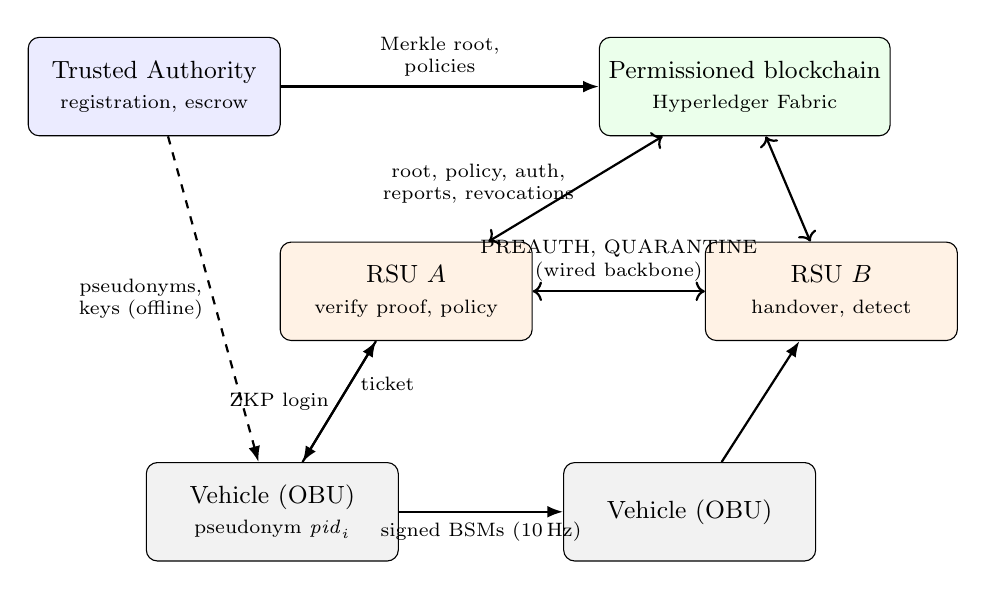
\begin{tikzpicture}[
  box/.style={draw, rounded corners, align=center, minimum width=3.2cm, minimum height=1.25cm, font=\small},
  arr/.style={-{Latex[length=2mm]}, thick}, lab/.style={font=\scriptsize, align=center}]
  \node[box, fill=blue!8] (ta) at (0,4.2) {Trusted Authority\\\scriptsize registration, escrow};
  \node[box, fill=green!8] (ledger) at (7.5,4.2) {Permissioned blockchain\\\scriptsize Hyperledger Fabric};
  \node[box, fill=orange!10] (rsu1) at (3.2,1.6) {RSU $A$\\\scriptsize verify proof, policy};
  \node[box, fill=orange!10] (rsu2) at (8.6,1.6) {RSU $B$\\\scriptsize handover, detect};
  \node[box, fill=gray!10] (v1) at (1.5,-1.2) {Vehicle (OBU)\\\scriptsize pseudonym $\mathit{pid}_i$};
  \node[box, fill=gray!10] (v2) at (6.8,-1.2) {Vehicle (OBU)};
  \draw[arr] (ta) -- node[lab, above]{Merkle root,\\policies} (ledger);
  \draw[arr, dashed] (ta) -- node[lab, left]{pseudonyms,\\keys (offline)} (v1);
  \draw[arr] (v1) -- node[lab, left]{ZKP login} (rsu1);
  \draw[arr] (rsu1) -- node[lab, right, pos=0.35]{ticket} (v1);
  \draw[arr, <->] (rsu1) -- node[lab, left, pos=0.55]{root, policy, auth,\\reports, revocations} (ledger);
  \draw[arr, <->] (rsu2) -- (ledger);
  \draw[arr, <->] (rsu1) -- node[lab, above]{PREAUTH, QUARANTINE\\(wired backbone)} (rsu2);
  \draw[arr] (v1) -- node[lab, below]{signed BSMs (10\,Hz)} (v2);
  \draw[arr] (v2) -- (rsu2);
\end{tikzpicture}
\caption{Entities and the information each exchanges. The blockchain holds only state that several
RSUs must share and that must be auditable; it is not on the path of individual safety messages.}
\label{fig:architecture}
\end{figure}

Figure~\ref{fig:architecture} shows the entities. The guiding principle of the design is that
\emph{proofs are verified at the edge and the ledger stores only shared state}. An RSU verifies a
zero-knowledge proof locally in well under a millisecond, while a Fabric commit takes hundreds of
milliseconds (Section~\ref{sec:res-ledger}). So the ledger is read from a local, regularly
synchronised copy, written asynchronously, and never waited for while a safety message is handled.
The ledger stores:
\begin{itemize}
  \item the Merkle root of each registration epoch (never a per-vehicle record);
  \item service policies: which vehicle classes may use which service;
  \item authorization records keyed by pseudonym, so that the next RSU can accept a handover;
  \item misbehaviour reports with evidence hashes, and the revocation list;
  \item trace requests and the RSU organizations' approvals for identity reveal.
\end{itemize}

\section{Registration}

For each vehicle $v$ the TA generates $P$ pseudonyms (5 by default), each a fresh key pair
$(x_i, Y_i = x_i G)$ with a random 64-bit identifier $\mathit{pid}_i$, and the vehicle's class
(\textit{car}, \textit{truck} or \textit{emergency}). It builds the Merkle tree over the leaves of
all pseudonyms of all vehicles, in shuffled order so that positions do not reveal which pseudonyms
belong together, and gives each vehicle its keys and Merkle paths over a secure channel. It publishes
the root with its validity period on the ledger through the chaincode function
\texttt{RegisterRoot}. Finally it encrypts the vehicle's identity record (identity and list of
pseudonyms) and escrows the key with the RSU organizations as $t$-of-$n$ Shamir shares, with
$t = 2f+1$ for $n = 3f+1$ organizations (5 of 9 in the evaluated scenarios).

\section{Authentication}

\begin{figure}[htbp]\centering
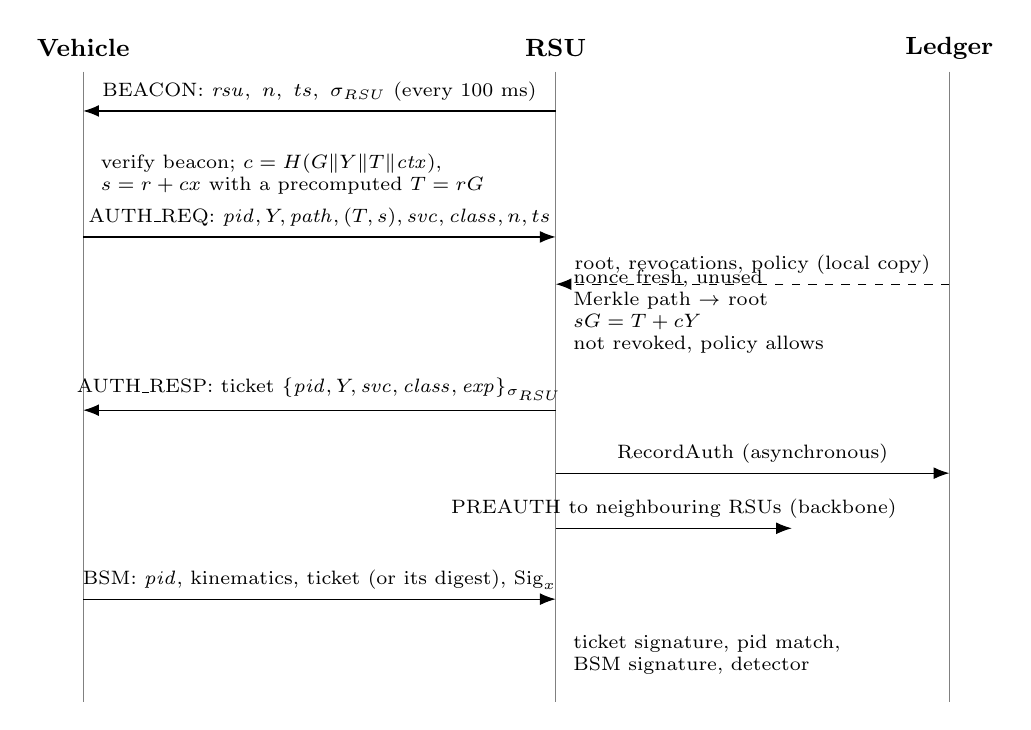
\begin{tikzpicture}[font=\small, >={Latex[length=2mm]}]
  \node (v) at (0,0) {\textbf{Vehicle}};
  \node (r) at (6,0) {\textbf{RSU}};
  \node (l) at (11,0) {\textbf{Ledger}};
  \draw[gray] (0,-0.3) -- (0,-8.3); \draw[gray] (6,-0.3) -- (6,-8.3); \draw[gray] (11,-0.3) -- (11,-8.3);
  \draw[->] (6,-0.8) -- node[above, font=\scriptsize]{BEACON: $\mathit{rsu},\ n,\ ts,\ \sigma_{RSU}$ (every 100 ms)} (0,-0.8);
  \node[align=left, font=\scriptsize, anchor=west] at (0.1,-1.6) {verify beacon; $c = H(G\|Y\|T\|\mathit{ctx})$,\\ $s = r + cx$ with a precomputed $T = rG$};
  \draw[->] (0,-2.4) -- node[above, font=\scriptsize]{AUTH\_REQ: $\mathit{pid}, Y, \mathit{path}, (T,s), \mathit{svc}, \mathit{class}, n, ts$} (6,-2.4);
  \node[align=left, font=\scriptsize, anchor=west] at (6.1,-3.35) {nonce fresh, unused\\ Merkle path $\to$ root\\ $sG = T + cY$\\ not revoked, policy allows};
  \draw[dashed, ->] (11,-3.0) -- node[above, font=\scriptsize]{root, revocations, policy (local copy)} (6,-3.0);
  \draw[->] (6,-4.6) -- node[above, font=\scriptsize]{AUTH\_RESP: ticket $\{\mathit{pid}, Y, \mathit{svc}, \mathit{class}, \mathit{exp}\}_{\sigma_{RSU}}$} (0,-4.6);
  \draw[->] (6,-5.4) -- node[above, font=\scriptsize]{RecordAuth (asynchronous)} (11,-5.4);
  \draw[->] (6,-6.1) -- node[above, font=\scriptsize]{PREAUTH to neighbouring RSUs (backbone)} (9,-6.1);
  \draw[->] (0,-7.0) -- node[above, font=\scriptsize]{BSM: $\mathit{pid}$, kinematics, ticket (or its digest), $\mathrm{Sig}_{x}$} (6,-7.0);
  \node[align=left, font=\scriptsize, anchor=west] at (6.1,-7.7) {ticket signature, pid match,\\ BSM signature, detector};
\end{tikzpicture}
\caption{Authentication, ticket issue and the first safety message}\label{fig:auth-seq}
\end{figure}

Figure~\ref{fig:auth-seq} shows the exchange.
\begin{enumerate}
  \item Every RSU broadcasts a signed beacon every 100\,ms with its identity, a fresh nonce $n$ and a
  timestamp. A vehicle accepts only beacons from RSUs whose public keys it holds.
  \item The vehicle computes the Schnorr response for the current pseudonym with
  \[\mathit{ctx} = \mathsf{enc}(\texttt{"VANET-AUTH-v1"}, \mathit{rsu}, n, ts, \mathit{svc}, \mathit{pid}, \mathit{class})\]
  and sends the pseudonym, its public key, the Merkle path, the proof, the requested service and its
  class.
  \item The RSU checks that the nonce is one it issued recently and that this (nonce, pseudonym) pair
  was not used before, rebuilds the leaf and verifies the path against the current root from the
  ledger, verifies the proof, checks that the pseudonym is neither revoked nor quarantined, and
  evaluates the authorization predicate
  \begin{equation}\label{eq:access}
    \mathrm{Access}(v, \mathit{svc}) = 1 \iff \mathrm{Verify}(\pi, Y) = 1 \;\wedge\; \mathit{pid} \notin \mathit{RL}
      \;\wedge\; \mathit{class} \in \mathrm{Policy}(\mathit{svc}).
  \end{equation}
  \item If access is granted, the RSU signs a ticket over the pseudonym, its key, the service, the
  class, its own identity and an expiry 30\,s ahead, records the authorization on the ledger
  asynchronously, and sends a signed PREAUTH note over the backbone to its neighbouring RSUs.
\end{enumerate}
The RSU learns the pseudonym, the class and that the vehicle is registered, and nothing else: the
leaf of another vehicle of the same class looks the same, the proof is zero-knowledge, and the
Merkle path reveals only the leaf position, which is shuffled.

\section{Handover and Pseudonym Change}

When a vehicle approaches the edge of its RSU's range (80\,\% of the nominal 300\,m) and hears a
closer RSU, or loses its RSU, it sends a handover request with its ticket, signed with the ticket key
and bound to the new RSU's beacon nonce. The new RSU checks the issuing RSU's signature on the ticket,
the request signature and the shared authorization: either the authorization record on the ledger or,
if the commit has not reached its local copy yet, the PREAUTH note from the issuing RSU. A handover
needs no new proof. After three sessions a vehicle switches to its next pseudonym and authenticates
afresh, so that a pseudonym's lifetime stays short.

\section{Safety Messages}

Each BSM carries the pseudonym, the kinematic fields and the ticket, and is signed with the
pseudonym's secret key, whose public key is in the ticket. A receiver checks the ticket's RSU
signature, that the ticket's pseudonym matches, the BSM signature and the ticket expiry. The receiver
needs no certificate chain and no ledger access. In Phase~I every BSM carries the full ticket, which
makes it about 330 bytes.

\section{Misbehaviour Detection and Reporting}\label{sec:detect}

Every RSU runs a detector on each authentic BSM against that pseudonym's recent history. Hard
plausibility rules flag positions beyond radio range, speeds above 60\,m/s, accelerations above the
physical limit, positions inconsistent with the claimed speed, impossible heading flips, replays and
message rates above 13 per second. Weak rules (sudden appearance close to the RSU, two pseudonyms at
the same place) count only in pairs. An RSU reports a pseudonym once $K = 3$ of its last $W = 10$
messages were flagged, with the hash of a flagged, \emph{signed} message as evidence, through the
chaincode function \texttt{ReportMisbehaviour}.

\section{Revocation and Threshold Identity Reveal}

The chaincode revokes a pseudonym automatically once two distinct RSUs have reported it. A single
report, perhaps a detector error, therefore has no effect. RSUs see the revocation through their
local ledger copy and reject the pseudonym's BSMs and logins. An RSU that reported a now-revoked
pseudonym opens a trace request on the ledger (\texttt{RequestTrace}), and the RSU organizations
approve it (\texttt{ApproveTrace}). Once $t$ approvals are recorded, each approving organization
releases its key share, the TA reconstructs the escrow key, decrypts the identity record and revokes
all of the vehicle's pseudonyms. The vehicle's next login attempt fails and it is shut out. No single
party can unmask a vehicle: the TA lacks the key, and fewer than $t$ RSU organizations hold too few
shares.

\section{Ledger Interface}

\begin{table}[htbp]\centering\small
\caption{Chaincode functions and who may call them}\label{tab:chaincode}
\begin{tabular}{@{}llp{7.2cm}@{}}
\toprule
Function & Caller & Effect \\
\midrule
\texttt{RegisterRoot} & TA & publish the Merkle root of an epoch \\
\texttt{SetPolicy}, \texttt{SetConfig} & TA & classes allowed per service; $K$, trace threshold \\
\texttt{RecordAuth} & RSU & authorization record of a pseudonym (rejected if revoked) \\
\texttt{ReportMisbehaviour} & RSU & report with evidence hash; revoke at $K$ reporters \\
\texttt{Revoke} & TA & revoke pseudonyms after a trace \\
\texttt{RequestTrace}, \texttt{ApproveTrace} & RSU & open and approve an identity reveal \\
\texttt{SetReporterWeight} & TA & report weight of an RSU (Section~\ref{sec:trust}) \\
\texttt{IsRevoked}, \texttt{GetRoot}, \ldots & any & queries; \texttt{ListRevokedSince} for synchronisation \\
\bottomrule
\end{tabular}
\end{table}

Table~\ref{tab:chaincode} lists the chaincode functions. The chaincode reads the caller's role from
its Fabric certificate, so an RSU cannot change a policy and a vehicle cannot write at all. RSUs reach
Fabric through a REST gateway that signs each transaction with the caller's identity.

\section{Security Analysis}

\begin{itemize}
  \item \textbf{Impersonation.} An accepting proof requires $x_i$ for a leaf in the registered tree
  (soundness of the Schnorr proof and collision resistance of the hash). A signed BSM requires the
  key in an RSU-signed ticket.
  \item \textbf{Replay.} A login proof is bound to the RSU, a nonce the RSU issued within the
  freshness window and the pseudonym, and each (nonce, pseudonym) pair is accepted once. BSMs carry a
  timestamp and sequence number that the detector checks; handover requests are bound to the new
  RSU's nonce.
  \item \textbf{Class and service escalation.} The class is part of the Merkle leaf and of the proof
  context, so claiming another class breaks verification; the policy check (\ref{eq:access}) then
  decides the service.
  \item \textbf{Anonymity.} RSUs and vehicles see pseudonyms only, and the proof is zero-knowledge.
  Linking pseudonyms of one vehicle requires its escrow record, which needs $t$ organizations.
  \item \textbf{Accountability.} Every revocation and every reveal is a ledger transaction signed by
  identified organizations, and the ledger is append-only.
  \item \textbf{Limitations.} The TA knows at registration which pseudonyms belong to which vehicle.
  The RSUs learn which pseudonym was where, and a global eavesdropper can link consecutive pseudonyms
  by position. The privacy profile of Chapter~\ref{ch:opt} addresses both.
\end{itemize}

\chapter{Implementation}\label{ch:impl}

The system is implemented in Python (protocol, simulation glue, detection and evaluation), Go
(chaincode) and JavaScript (ledger gateway and live map). Everything is in one repository and runs
from a Makefile. This chapter describes the parts and how they connect.

\section{Overview}

\begin{figure}[htbp]\centering
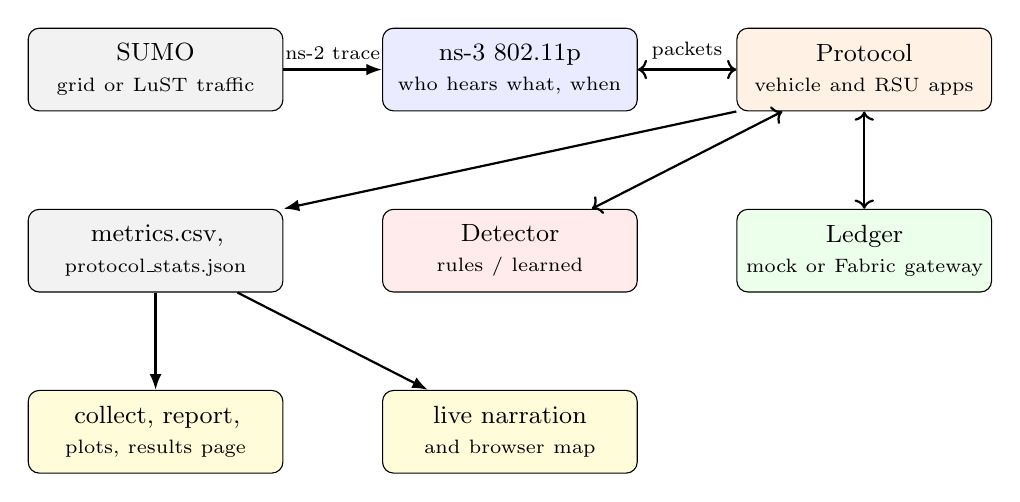
\begin{tikzpicture}[
  box/.style={draw, rounded corners, align=center, minimum height=1.05cm, text width=3.0cm, font=\small},
  arr/.style={-{Latex[length=2mm]}, thick}]
  \node[box, fill=gray!10] (sumo) at (0,0) {SUMO\\\scriptsize grid or LuST traffic};
  \node[box, fill=blue!8] (ns3) at (4.5,0) {ns-3 802.11p\\\scriptsize who hears what, when};
  \node[box, fill=orange!10] (proto) at (9,0) {Protocol\\\scriptsize vehicle and RSU apps};
  \node[box, fill=green!8] (ledger) at (9,-2.3) {Ledger\\\scriptsize mock or Fabric gateway};
  \node[box, fill=red!8] (det) at (4.5,-2.3) {Detector\\\scriptsize rules / learned};
  \node[box, fill=gray!10] (metrics) at (0,-2.3) {metrics.csv,\\\scriptsize protocol\_stats.json};
  \node[box, fill=yellow!15] (eval) at (0,-4.6) {collect, report,\\\scriptsize plots, results page};
  \node[box, fill=yellow!15] (viz) at (4.5,-4.6) {live narration\\\scriptsize and browser map};
  \draw[arr] (sumo) -- node[above, font=\scriptsize]{ns-2 trace} (ns3);
  \draw[arr, <->] (ns3) -- node[above, font=\scriptsize]{packets} (proto);
  \draw[arr, <->] (proto) -- (ledger);
  \draw[arr, <->] (proto) -- (det);
  \draw[arr] (proto.south west) -- (metrics.north east);
  \draw[arr] (metrics) -- (eval);
  \draw[arr] (metrics) -- (viz);
\end{tikzpicture}
\caption{Simulation and evaluation pipeline}\label{fig:pipeline}
\end{figure}

Figure~\ref{fig:pipeline} shows the pipeline. SUMO~\cite{lopez2018sumo} decides where every vehicle drives. ns-3 models
the radio: transmission, propagation, collisions and the MAC. The protocol code runs inside every
vehicle and RSU node and talks to the ledger and the detector. Every event is logged to
\texttt{metrics.csv}, from which the evaluation computes all results. Table~\ref{tab:code} lists
the main parts of the code.

\begin{table}[htbp]\centering\small
\caption{Code organisation}\label{tab:code}
\begin{tabular}{@{}lp{10.5cm}@{}}
\toprule
Folder & Contents \\
\midrule
\texttt{mobility/} & grid and LuST scenario builders, SUMO-to-ns-2 trace conversion, RSU placement \\
\texttt{network/} & scenario runner, ns-3 radio backend, node hooks, metrics, ledger bridge, live map \\
\texttt{protocol/} & vehicle and RSU logic, cryptography, message encoding, registration, escrow, TESLA, ECQV, Bloom filter, batch verification, V2V verifier, simulator glue \\
\texttt{ledger/} & Fabric network scripts, Go chaincode, Node.js REST gateway, mock ledger, conformance tests, load benchmark \\
\texttt{detection/} & detector (rules, features, learned models), VeReMi loaders, benchmark and training \\
\texttt{experiments/} & sweep configurations, runner, collection, reports, plots, results page, tracker attack \\
\bottomrule
\end{tabular}
\end{table}

\section{Mobility}

\textbf{Grid.} A $5\times5$ junction grid with 250\,m blocks (1\,km$^2$) and two lanes per
direction. Random trips start during the first half of the run, so vehicles enter one after another.
Nine RSUs stand 450\,m apart, each with a nominal range of 300\,m, so ranges overlap.

\textbf{LuST.} The Luxembourg SUMO Traffic scenario~\cite{codeca2015lust} models a full day of the
city's traffic. The evaluation simulates the whole city and cuts a 1.35\,km\,$\times$\,1.35\,km box
in the centre at three times of day: 06:00 (about 150 vehicles in the box), 14:00 (about 260) and the
08:00 peak (about 525). A 900\,s warm-up fills the roads before the measured window. Vehicles that
leave the box are parked outside radio range until they come back.

\textbf{Mobility step and lane changes.} SUMO runs at 0.1\,s steps. Its default instant lane change
is a 3.2\,m sideways jump in one step, which the trace turned into a false 32\,m/s velocity that the
detector rightly flagged. The evaluation therefore uses a 2\,s lane-change duration, as real drivers
do, which removed all such spikes on the grid and all but two of 385 on LuST.

\section{Radio Network}

\begin{table}[htbp]\centering\small
\caption{IEEE 802.11p parameters in ns-3}\label{tab:radio}
\resizebox{\textwidth}{!}{%
\begin{tabular}{@{}lp{9cm}@{}}
\toprule
Parameter & Value \\
\midrule
Standard, band & IEEE 802.11p (WAVE), 5.9\,GHz, 10\,MHz channel \\
Data rate & 6\,Mb/s \\
Transmit power, receiver sensitivity & 20\,dBm, $-85$\,dBm \\
Propagation & log-distance, exponent 2.196, 47.86\,dB at 1\,m \\
Nominal range & 400\,m \\
Access categories & BSMs, beacons and TESLA keys on AC\_VO; the rest on AC\_BE \\
Wired RSU backbone & 2\,ms latency \\
\bottomrule
\end{tabular}}
\end{table}

ns-3 (version 3.44~\cite{riley2010ns3}) is driven from Python through its cppyy bindings.
Table~\ref{tab:radio} lists the radio configuration. A lighter pure-Python backend with the same
parameters exists for development and unit tests; every reported result comes from ns-3. ns-3's
FlowMonitor and the PHY's busy time give the delivery ratio and the channel busy ratio, sampled every
second at each RSU.

\section{Protocol}

The protocol package implements Chapter~\ref{ch:design}. Schnorr signatures and
proofs use \texttt{coincurve} (libsecp256k1), and the escrow uses AES-GCM~\cite{nist80038d} from
\texttt{cryptography}. Messages use a compact binary encoding: one byte per field
name from an append-only table, binary hex strings, and 16-byte packed kinematics. Vehicles and RSUs
are applications attached to ns-3 nodes through a small set of hooks: send, schedule, position, log
and the local ledger copy.

\textbf{Processing time.} Simulated time does not advance while Python computes. Instead, the cost of
every cryptographic operation was measured on the real implementations
(Table~\ref{tab:compute}) and is charged as processing delay. With \emph{per-node processor} modelling, each
RSU and vehicle has one processor that executes this work in arrival order. Latency therefore
includes queueing, and a BSM that would wait more than 100\,ms is dropped as too old to be useful.
Vehicle processors are assumed five times slower than the development PC, an AMD Ryzen~7 4800H. A
sensitivity sweep varies this factor (Section~\ref{sec:res-sens}).

\gentab{tab_compute}

\textbf{Vehicle-side verification.} Each vehicle verifies the BSMs of senders within 100\,m on its
own processor, as a receiver that acts on them would. It caches tickets learned from full-ticket BSMs
of farther senders.

\section{Ledger}

The chaincode is written in Go for Hyperledger Fabric~3.1.5 and deployed on a Fabric network with two
peer organizations and an ordering service of one Raft orderer or four SmartBFT orderers. A Node.js
gateway exposes it as a REST interface. It maps an \texttt{X-Identity} header to the caller's Fabric
certificate, signs transactions, reports endorsement and commit times, and keeps an activity log. An
HTTP conformance suite runs unchanged against the real gateway and against a mock with the same
rules. For long parameter sweeps, the simulator uses an in-process ledger with the same functions
and a 500\,ms commit delay, which is the Raft commit time measured with the default batch timeout
(Section~\ref{sec:res-ledger}). RSUs read from a local copy that is updated every second, or at the
mock's commit time.

\section{Detection}

The detector computes per-message plausibility features against the pseudonym's history: implied
speed, speed and position consistency over 0.8--3\,s baselines, acceleration, heading change,
message rate, distance from the RSU, the signal-strength distance and sequence numbers. It applies the
rules of Section~\ref{sec:detect}. For comparison, learned models over the same features (a random
forest and gradient-boosted trees~\cite{friedman2001gbm} with a history window, built with
scikit-learn~\cite{pedregosa2011sklearn}) are trained and tested on VeReMi
Extension~\cite{kamel2020veremiext}, on five vehicle-disjoint splits so that no vehicle's messages
appear in both training and test data. The scheme itself uses the rules and the signal-strength
check, which do not depend on the road network.

\section{Evaluation Framework}\label{sec:eval-framework}

A sweep is a JSON configuration: fixed options, a grid of parameters (for example 50, 100 and 150
vehicles), the variants to compare and the seeds. The runner executes every combination in parallel
and skips finished runs. A collection step turns each run's event log into about 100 metrics. The
report step computes means with 95\,\% confidence intervals over the seeds and Welch's
t-test~\cite{welch1947} against each baseline, and writes Markdown and LaTeX tables, PNG, PDF and SVG
figures, and an interactive results page. The tables and numbers in this report are generated from
the same outputs (Appendix~\ref{app:repro}).

\textbf{Baselines.} Two baselines run on the same simulator. \emph{ECDSA-PKI} represents IEEE
1609.2-style pseudonym certificates: the vehicle presents a CA-signed certificate and signs with
ECDSA~\cite{johnson2001ecdsa} P-256, using the measured ECDSA costs. \emph{Central-TA} sends every login over the backbone
to one central authority that decides and answers.

\textbf{Tracker.} For privacy, a global eavesdropper records every BSM. A tracker then tries to link
each new pseudonym to a disappearing one by predicting positions from the last speed and heading. The
metrics are the share of pseudonym changes linked correctly and the share of a trip that can be
followed from start to end.

\section{Live Demonstration Tools}

Two tools show a run as it happens. A terminal narration prints each important event in plain
language, with a one-line explanation the first time each kind appears, and a status line every five
simulated seconds. A live map in the browser (Figure~\ref{fig:livemap}) draws the SUMO road network,
the RSUs with their coverage and every vehicle, coloured by its state. Clicking a vehicle shows its
pseudonym, class, ticket, revocation state and recent events. Clicking an RSU shows its load, the
vehicles in range, its counters and its recent checks. The page can pause the simulation and change
its speed.

\begin{figure}[htbp]\centering
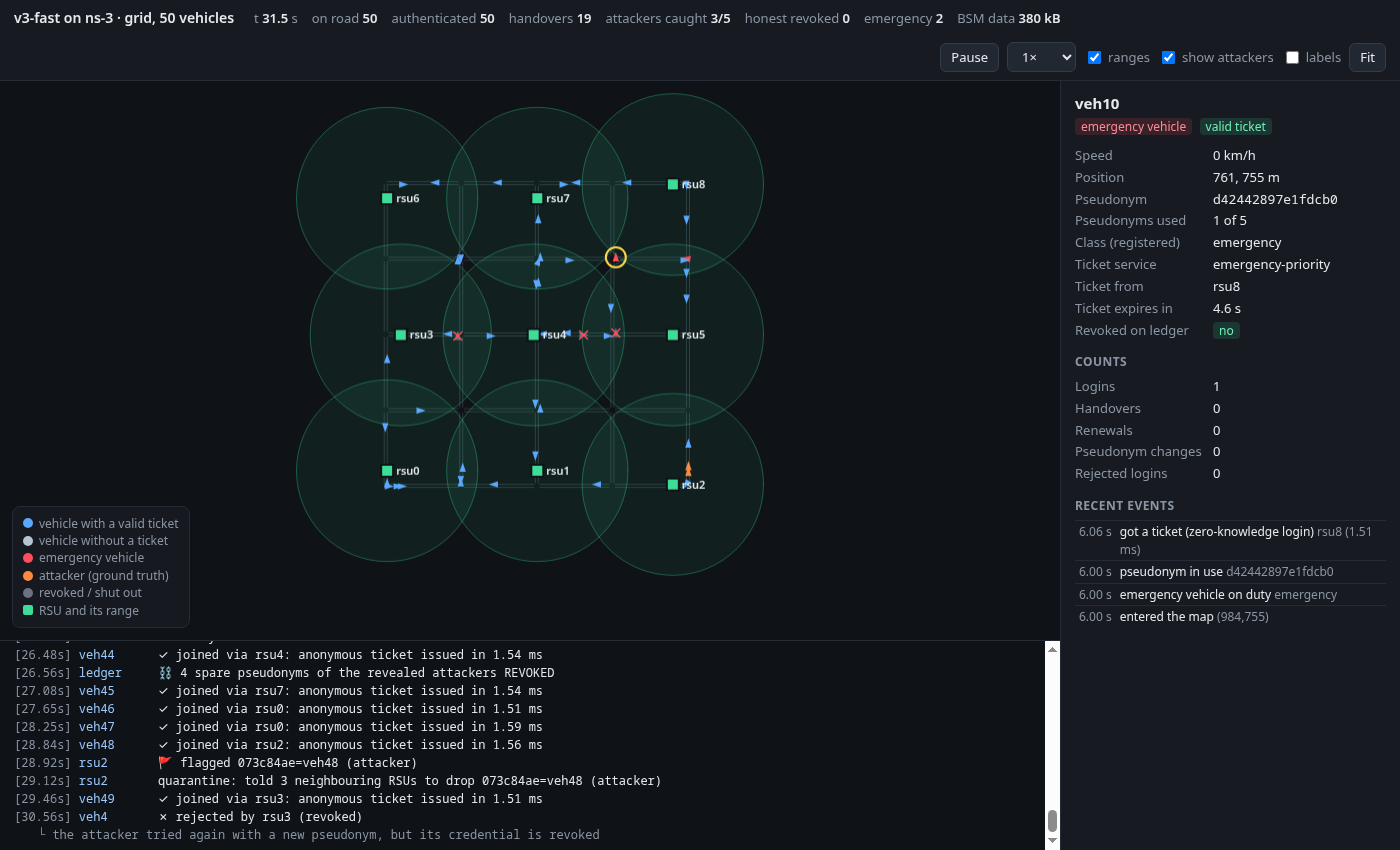
\includegraphics[width=0.85\textwidth]{figures/live_map_vehicle.png}
\caption{Live map of a running ns-3 simulation (grid, 50 vehicles, with emergency vehicles).
The selected emergency vehicle shows its registered class and its \texttt{emergency-priority}
ticket; revoked attackers are marked with a cross; the feed narrates detection and revocation.}
\label{fig:livemap}
\end{figure}

\section{Testing}

178 automated tests cover the cryptographic primitives, message encoding, the protocol flows
(including replay, forged tickets, swapped certificate requests, class escalation and fake emergency
alerts), the detector, the ledger rules and the processor model. The chaincode has its own Go unit
tests, and the gateway passes the HTTP conformance suite.

\chapter{Results and Discussion}\label{ch:results}

This chapter reports the evaluation. All network results come from ns-3. Each configuration runs with
several seeds, which change SUMO's trips, the choice of attackers and the radio's randomness. Tables
give the mean and the 95\,\% confidence interval over the seeds.

\section{Experimental Setup}

\begin{table}[htbp]\centering\small
\caption{Common parameters of the network experiments}\label{tab:setup}
\resizebox{\textwidth}{!}{%
\begin{tabular}{@{}lp{8.5cm}@{}}
\toprule
Parameter & Value \\
\midrule
Simulated time per run & 120\,s (180\,s for the compromised RSUs, 60\,s on LuST) \\
Scenarios & grid with 50, 100, 150 vehicles; LuST at 06:00, 14:00, 08:00 \\
RSUs & 9 (grid, 450\,m apart), 300\,m nominal range \\
Seeds & 5 (grid comparison), 10 (compromised RSUs), 3 (others) \\
Attackers & 10\,\% of the vehicles, random position offsets from 30\,s \\
Reports to revoke ($K$), reveal threshold & 2 RSUs; 5 of 9 organizations \\
Ticket lifetime, pseudonyms per vehicle & 30\,s; 5 (20 with mix zones) \\
Ledger in sweeps & in-process, 500\,ms commit (Section~\ref{sec:res-ledger}) \\
Processors & RSU at measured speed, vehicle 5$\times$ slower \\
Vehicle verification & BSMs of senders within 100\,m \\
\bottomrule
\end{tabular}}
\end{table}

Table~\ref{tab:setup} lists the common parameters. The compared variants are the Phase~I scheme, its
optimised profiles (Table~\ref{tab:profiles}) and the two baselines of Section~\ref{sec:eval-framework}.

\textbf{Metrics.}
\begin{itemize}
  \item \emph{Ticket}: time from sending a login (or renewal) to holding a valid ticket. \emph{Ticket
  after 10\,s} leaves out the start of a run.
  \item \emph{Safety traffic}: BSM and TESLA-key bytes per vehicle per second.
  \item \emph{PDR}: share of broadcasts received by the nodes within 300\,m of the sender.
  \item \emph{CBR}: channel busy ratio measured at the RSUs.
  \item \emph{V2V accept}: time from sending a BSM to a neighbouring vehicle accepting it.
  \item \emph{Revoked accepted}: share of BSMs from revoked senders that vehicles still accepted.
  \item \emph{Caught}: share of attackers reported to the ledger.
  \item \emph{Honest revoked}: honest vehicles that lost a pseudonym to revocation.
  \item \emph{Tracked}: share of pseudonym changes the eavesdropper links correctly.
\end{itemize}

\section{Comparison on the Grid}\label{sec:res-grid}

\gentab{tab_compare}
\gentab{tab_compare_sec}

Tables~\ref{tab:compare} and~\ref{tab:compare-sec} compare all variants at \R{cmp}{vehicles}
vehicles, and Figure~\ref{fig:grid} shows the trends over vehicle density.

\textbf{Latency.} The Phase~I scheme issues a ticket in \R{cmp/Phase-I}{ticket_ms_mean}\,ms,
v3-fast in \R{cmp/v3-fast}{ticket_ms_mean}\,ms (\R{cmp/derived}{ticket_ms_mean_cut_pct}\,\% less),
and the ECDSA-PKI baseline in \R{cmp/ECDSA-PKI}{ticket_ms_mean}\,ms. The zero-knowledge login is
therefore as fast as presenting a certificate. Centralising the decision (Central-TA) costs
\R{cmp/Central-TA}{ticket_ms_mean}\,ms, because every login crosses the backbone and queues at one
authority. A vehicle accepts a neighbour's BSM after \R{cmp/v3-fast}{v2v_accept_ms_mean}\,ms with
v3-fast against \R{cmp/Phase-I}{v2v_accept_ms_mean}\,ms with Phase-I: smaller messages spend less
time on the air, and the vehicle processor has less to verify.

\textbf{Channel load.} This is the largest effect. Phase-I's \R{cmp/Phase-I}{bsm_bytes}-byte BSMs at
10\,Hz put \R{cmp/Phase-I}{safety_bytes_per_vehicle_s}\,B/s per vehicle on the channel. v3-fast sends
\R{cmp/v3-fast}{safety_bytes_per_vehicle_s}\,B/s, \R{cmp/derived}{safety_factor} times less, by
combining smaller messages with dead-reckoning triggering. The channel busy ratio falls from
\R{cmp/Phase-I}{cbr_rsu_mean} to \R{cmp/v3-fast}{cbr_rsu_mean}, and the delivery ratio rises from
\R{cmp/Phase-I}{pdr} to \R{cmp/v3-fast}{pdr} because fewer frames collide.

\textbf{Revocation.} Without information from the ledger, vehicles in Phase-I accepted every BSM from
revoked senders (\R{cmp/Phase-I}{v2v_revoked_accepted_ratio}). With the revocation filter in RSU
beacons, v3-fast vehicles accepted \R{cmp/v3-fast}{v2v_revoked_accepted_ratio}. Every variant caught
every attacker, and no honest vehicle was revoked.

\textbf{Privacy.} Without mix zones, the eavesdropper links \R{cmp/v3-fast}{tracking_success} of the
pseudonym changes, because a pseudonym change alone does not hide a vehicle's trajectory. v3-private
lowers this to \R{cmp/v3-private}{tracking_success}, at the price of a ticket time of
\R{cmp/v3-private}{ticket_ms_mean}\,ms, the cost of the BBS proof.

\gentab{tab_significance}

Table~\ref{tab:significance} tests the differences: a bold entry means that the difference between
the challenger and Phase-I is significant at the 5\,\% level (Welch's t-test over the seeds).

\begin{figure}[htbp]\centering
\genfig[\textwidth]{grid_overview}
\caption{Grid scenario over vehicle density (mean and 95\,\% CI over 5 seeds)}\label{fig:grid}
\end{figure}

\gentab{tab_compare_all}

\section{Real Traffic: LuST}\label{sec:res-lust}

\gentab{tab_lust}

\begin{figure}[htbp]\centering
\genfig[\textwidth]{lust_overview}
\caption{LuST traffic at three times of day (mean and 95\,\% CI over 3 seeds)}\label{fig:lust}
\end{figure}

Table~\ref{tab:lust} and Figure~\ref{fig:lust} repeat the comparison of Phase-I and v3-fast on real
Luxembourg traffic, with 60\,s runs, since a run of the 08:00 peak with over 800 vehicles takes more
than an hour to simulate. Two differences from the grid
matter. First, a cut of real traffic starts with hundreds of vehicles already on the road, which all
log in during the first seconds. The RSUs' processors keep up (a login costs them well under a
millisecond), but the radio does not: hundreds of login requests of about 680 bytes, each with its
Merkle path and proof, and the RSUs' ticket responses compete for the channel and wait in the 802.11p
queues. In a 15\,s run of the 08:00 peak, a login request spent about 110\,ms and a ticket response
about 240\,ms on the air during the first three seconds. The mean ticket time therefore includes
this start-up burst. The ticket time after 10\,s shows the steady state: in the
08:00 peak, v3-fast issues tickets in \R{lust:peak/v3-fast}{ticket_ms_steady_mean}\,ms once the
burst has passed. Second, real roads with many lanes and junctions give more manoeuvres, so
dead-reckoning triggering saves less than on the grid. At the peak, v3-fast still puts
\R{lust:peak/v3-fast}{safety_bytes_per_vehicle_s}\,B/s per vehicle on the channel against
\R{lust:peak/Phase-I}{safety_bytes_per_vehicle_s}\,B/s for Phase-I, with channel busy ratios of
\R{lust:peak/v3-fast}{cbr_rsu_mean} and \R{lust:peak/Phase-I}{cbr_rsu_mean}.

Two results differ from the grid in v3-fast's disfavour. At the peak, its channel busy ratio is
above the 0.30 at which adaptive signing switches to TESLA, so a neighbour can accept a BSM only once
its key is disclosed: V2V acceptance takes \R{lust:peak/v3-fast}{v2v_accept_ms_mean}\,ms against
\R{lust:peak/Phase-I}{v2v_accept_ms_mean}\,ms for Phase-I. This is the price of a channel that still
delivers \R{lust:peak/v3-fast}{pdr} of the broadcasts, where Phase-I delivers
\R{lust:peak/Phase-I}{pdr}. Second, between 85 and 89\,\% of the attackers are caught on LuST,
for both variants, against all of them on the grid: the attack starts at 30\,s of a 60\,s run, and
an attacker that leaves the coverage of the RSUs before two of them have reported it is not revoked
in the run. No honest vehicle was revoked.

\section{Ablation: What Each Mechanism Contributes}\label{sec:res-ablation}

\gentab{tab_ablation}
\gentab{tab_ablation_sec}

Tables~\ref{tab:ablation} and~\ref{tab:ablation-sec} start from v2 and add one mechanism at a time. It separates the
mechanisms that reduce bytes on the air (TESLA, implicit certificates, dead reckoning) from those
that reduce latency or handovers (clusters, renewal, batch verification under load), and those that
change security properties (revocation filter, signal-strength check) or privacy (BBS, mix zones).
For example, TESLA alone brings the safety traffic from \R{abl/v2}{safety_bytes_per_vehicle_s} to
\R{abl/v2 +tesla}{safety_bytes_per_vehicle_s}\,B/s, dead reckoning alone to
\R{abl/v2 +dead-reckoning}{safety_bytes_per_vehicle_s}\,B/s, and the revocation filter alone lowers
the share of BSMs from revoked senders that vehicles accept from
\R{abl/v2}{v2v_revoked_accepted_ratio} to \R{abl/v2 +revocation-filter}{v2v_revoked_accepted_ratio}.
The learned detector in hybrid mode is listed for completeness. It is not part of the profiles: a model
trained on one road network flagged honest vehicles on another, whereas the rules and the
signal-strength check transfer across cities.

\section{Misbehaviour Detection}\label{sec:res-detect}

\gentab{tab_veremi}

On VeReMi Extension (\R{veremi}{messages} messages from \R{veremi}{vehicles} vehicles,
Table~\ref{tab:veremi}), the plausibility rules alone reach an F1 score of \R{veremi}{rules_f1} with
no false positives. They miss subtle attacks such as small constant offsets, which stay within
physical limits. Learned models over the same features reach \R{veremi}{rf_f1} (random forest~\cite{breiman2001rf}), and
gradient boosting with a history window \R{veremi}{hgb_window_f1} at a false-positive rate of
\R{veremi}{hgb_window_fpr}.

\gentab{tab_sensitivity_attack}
\gentab{tab_sensitivity_attackers}

In the simulation, Tables~\ref{tab:sensitivity-attack} and~\ref{tab:sensitivity-attackers} show
detection per attack type and for an increasing share of attackers. Every attack type is caught,
and no honest vehicle is revoked, up to 30\,\% attackers. The two-report rule matters here: a
single RSU's false alarm has no consequence, so honest vehicles keep their pseudonyms even when one
RSU misjudges them.

\section{Compromised RSUs}\label{sec:res-trust}

\gentab{tab_trust}

Table~\ref{tab:trust} lets a quarter of the RSUs report random honest pseudonyms every 5\,s. With
plain $K = 2$ counting, two compromised RSUs together can revoke an honest pseudonym. With
trust-weighted reports, an RSU's weight falls once investigations show its reports were wrong,
after which its reports no longer suffice to revoke anyone. Its first false reports still count,
so weighting does not bring the number of honest vehicles revoked to zero: it falls from 5.8 to
2.4 per run for v2, while every attacker is still caught.

\section{Privacy}\label{sec:res-privacy}

\gentab{tab_mixzone_tradeoff}

\begin{figure}[htbp]\centering
\genfig[\textwidth]{mixzone}
\caption{Mix zones: longest silent period (s) against tracking and silence}\label{fig:mixzone}
\end{figure}

Pseudonym changes alone do not stop a global eavesdropper. In the grid comparison, the tracker links
\R{cmp/v3-fast}{tracking_success} of the changes made without mix zones. Table~\ref{tab:mixzone-tradeoff}
varies the longest silent period of the cooperative mix zones. Longer silence makes linking harder,
but a silent vehicle is invisible to its neighbours, so the table also reports the share of time
vehicles were silent and the 95th percentile of the position error neighbours see. This is the
safety--privacy trade-off that a deployment has to set.

\section{Blockchain Performance}\label{sec:res-ledger}

\gentab{tab_ledger}

Table~\ref{tab:ledger} measures the real Fabric~3.1.5 network under a steady load of
\texttt{RecordAuth} transactions, the most frequent write. With Raft and Fabric's default 500\,ms
batch timeout, the median commit takes \R{ledger}{raft_500ms_5_p50}\,ms, dominated by waiting for the
block to be cut. With a 50\,ms timeout, Raft commits in \R{ledger}{raft_50ms_5_p50}\,ms and SmartBFT
in \R{ledger}{bft_50ms_5_p50}\,ms at 5 transactions per second. At 20 per second, Byzantine fault
tolerance costs more: SmartBFT's median rises to \R{ledger}{bft_50ms_20_p50}\,ms against
\R{ledger}{raft_50ms_20_p50}\,ms for Raft. No transaction failed. These latencies confirm the design
principle: a commit takes tens to hundreds of milliseconds, too slow for the path of a safety message,
but fast enough for authorization records and revocations, which the RSUs bridge with PREAUTH notes
and quarantine.

\section{Sensitivity to the Vehicle Processor}\label{sec:res-sens}

\gentab{tab_sensitivity_obu}

The speed of real on-board units varies widely: software implementations on embedded processors
verify tens of signatures per second, while units with a cryptographic accelerator verify thousands.
Instead of relying on a single assumed factor, Table~\ref{tab:sensitivity-obu} repeats the comparison
with vehicle processors as fast as the development PC, 5 times slower, and 10 times slower.

\section{Emergency Vehicles}\label{sec:res-emergency}

\gentab{tab_emergency}
\gentab{tab_emergency_sec}

\begin{figure}[htbp]\centering
\genfig[\textwidth]{emergency}
\caption{Emergency vehicles on LuST: ticket times and warning coverage}\label{fig:emergency}
\end{figure}

Tables~\ref{tab:emergency} and~\ref{tab:emergency-sec} evaluate the extension of Section~\ref{sec:emergency} on the 14:00 LuST
traffic (v3-fast, 60\,s runs), where
the start-up burst creates long radio queues at the RSUs. The first compares the ticket time of emergency vehicles with
that of all other vehicles, with and without the priority lane. The second reports the share of vehicles
within 300\,m of an emergency vehicle that held a verified alert from it at most 1\,s old, the alert
delay, and the outcome of the fake-emergency attack. The design requirement is that no fake alert is
ever accepted, and that every fake emergency login is denied by the policy or rejected because the
pseudonym is already quarantined.

\section{Comparison with Published Schemes}\label{sec:res-literature}

Published schemes report their results on different simulators, hardware and libraries, so their
numbers cannot be placed next to ours directly: BPA~\cite{li2024bpa}, for example, measured an
elliptic-curve point multiplication at 0.233\,ms, our implementation at 0.016\,ms. The usual fair
comparison counts the cryptographic operations of one authentication and prices them with one set
of unit costs. Table~\ref{tab:literature} does this with BPA's published unit costs, the only set
that covers all the schemes. For BPA, ZAMA~\cite{xi2022zama} and B-TSCA~\cite{wang2021btsca} it
copies the operation counts, times and message sizes that BPA publishes (its Tables 4 and 5). For
our scheme it counts the operations of the protocol in Chapter~\ref{ch:design} and prices only the
point multiplications and hashes, which dominate; the message sizes are measured in the ns-3 runs.

\begin{table}[htbp]\centering\small\setlength{\tabcolsep}{4pt}
\caption{Cost of one authentication and one re-authentication (handover), priced with BPA's unit
costs (point multiplication 0.233\,ms, hash 0.0055\,ms, pairing 4.756\,ms)}\label{tab:literature}
\resizebox{\ifdim\width>\textwidth\textwidth\else\width\fi}{!}{%
\begin{tabular}{lllrllrr}
\toprule
Scheme & Ledger on the & \multicolumn{2}{l}{Authentication} & \multicolumn{2}{l}{Re-authentication} &
\multicolumn{2}{l}{Messages (B)} \\
\cmidrule(lr){3-4}\cmidrule(lr){5-6}\cmidrule(lr){7-8}
 & login path & operations & ms & operations & ms & auth. & re-auth. \\
\midrule
ZAMA~\cite{xi2022zama} & no & $11E + 5M + \dots$ & 2.64 & $2E + \dots$ & 1.76 & 1200 & 472 \\
B-TSCA~\cite{wang2021btsca} & lookup & $6E + 2P + 4H + \dots$ & 10.11 & $6E + 2P + 2H + \dots$ & 10.10 & 72 & 136 \\
BPA~\cite{li2024bpa} & re-auth. & $8\mathit{PM} + 3H + \dots$ & 1.91 & $7\mathit{PM} + H + \dots$ & 1.65 & 386 & 240 \\
This work & no & $8\mathit{PM} + 15H$ & 1.95 & $10\mathit{PM} + 6H$ & 2.36 & 716 & 410 \\
\bottomrule
\end{tabular}}
\par\smallskip\parbox{\textwidth}{\scriptsize $\mathit{PM}$: point multiplication, $H$: hash, $E$: modular
exponentiation, $M$: modular multiplication, $P$: bilinear pairing; ``$\dots$'' are the cheaper
operations listed in~\cite{li2024bpa}. Rows 1--3 and their times are as published in~\cite{li2024bpa}
(its Table~5 gives 386\,B for BPA's authentication, its Figure~8 368\,B). This work: authentication
= vehicle checks the beacon (2\,PM) and proves (1\,PM), RSU checks the Merkle path (10\,H) and the
proof (2\,PM) and signs the ticket (1\,PM), vehicle checks the ticket (2\,PM); handover = vehicle
checks the beacon and signs the request (3\,PM), the new RSU checks the old ticket and the request
(4\,PM) and signs a new ticket (1\,PM), vehicle checks it (2\,PM). Message sizes: request plus
ticket response, measured in ns-3.}
\end{table}

The comparison is mixed, and Table~\ref{tab:literature} shows why. In computation our login is on a
par with BPA, which also builds on elliptic-curve operations (eight point multiplications each),
cheaper than ZAMA, whose zero-knowledge proof uses modular exponentiations, and about five times
cheaper than B-TSCA, whose two pairings alone cost 9.5\,ms. Our messages are larger: the Merkle path
(nine hashes, 288\,B) travels with every proof, which is what lets the RSU check membership without
learning which registered vehicle it is talking to. Our handover costs more than BPA's
re-authentication, because the new RSU checks a signed ticket and a signed request instead of
looking up a shared trust key; RSU clusters (Section~\ref{sec:res-ablation}) avoid most of these
handovers instead.

The largest difference is architectural. BAAIoV~\cite{alsaeed2025baaiov} authenticates every vehicle
through a Hyperledger Fabric transaction and reports 150\,ms at 50 vehicles rising to 187\,ms at
150 vehicles, measured with SUMO and Fabric but without a radio model. Our design keeps the ledger
off the login path: on the grid with 150 vehicles a login completes in
\R{cmp/v3-fast}{ticket_ms_mean}\,ms end to end over 802.11p, while the ledger records it in the
background in the tens to hundreds of milliseconds that Table~\ref{tab:ledger} measures.
The two blockchain-and-ZKP schemes closest to ours, Wang et~al.~\cite{wang2025privacy} and the
emergency-vehicle scheme of Li et~al.~\cite{li2026emergency}, are compared in Chapter~\ref{ch:lit}
by their properties only.

\section{Discussion}

The research question of the Phase~I review asked whether ZKP authentication combined with
permissioned-blockchain authorization can work without unacceptable latency, computation or
communication overhead. On the measured network the answer is yes, under two conditions. First, the
ledger must stay off the safety-message path. Proofs are verified at the RSU in a fraction of a
millisecond, while ledger commits take tens to hundreds of milliseconds and are bridged by
PREAUTH and quarantine. Second, per-message authentication must be cheap. The Phase~I design was
dominated by its 330-byte BSMs; the optimised profile is \R{cmp/derived}{safety_factor} times lighter
on the channel and faster than the certificate baseline, without weakening the security model.

\textbf{Threats to validity.}
\begin{itemize}
  \item Radio and traffic are simulated. ns-3 and SUMO are the accepted tools for this purpose, and
  LuST adds real traffic, but no field test was done.
  \item Processing costs were measured on a PC and scaled for vehicles. The processor sensitivity
  sweep bounds the effect.
  \item The parameter sweeps use an in-process ledger with the measured Raft commit time, and the
  real Fabric network was measured separately on one machine. A wide-area deployment adds network
  latency to commits.
  \item The investigation that drives trust weights is simulated with ground truth.
  \item Attackers follow the VeReMi attack types and a fake-emergency attack. Adaptive attackers who
  stay just inside the plausibility limits are harder to detect, as the VeReMi results for small
  offsets show.
\end{itemize}

\chapter{Conclusion and Future Work}\label{ch:conclusion}

\section{Summary}

This project designed, implemented and evaluated privacy-preserving authentication and authorization
for VANETs that combines zero-knowledge proofs with a permissioned blockchain:
\begin{itemize}
  \item Vehicles prove registration and class with a Schnorr proof against a Merkle root on the
  ledger, bound to the RSU, a fresh nonce and the requested service.
  \item RSUs decide access with ledger policies and issue short-lived tickets.
  \item Misbehaving pseudonyms are reported to the ledger and revoked by two reports.
  \item A threshold of RSU organizations can unmask a revoked vehicle.
  \item The ledger is kept off the safety-message path.
\end{itemize}
The complete system runs on ns-3 with SUMO mobility on a grid and on real Luxembourg traffic, with
measured cryptographic costs, against certificate-based and centralised baselines and published
schemes. Its login is as fast as presenting a certificate and costs about as much computation as
BPA, and it puts \R{cmp/derived}{safety_factor} times less safety traffic on the channel than
certificate-signed messages. Its revocation filter lets vehicles, not only RSUs, ignore
revoked senders. On VeReMi Extension, the detector improves from an F1 score of \R{veremi}{rules_f1}
to \R{veremi}{hgb_window_f1}. Emergency vehicles are supported as a policy-restricted class whose
alerts cannot be forged under a normal ticket.

\section{Limitations}

\begin{itemize}
  \item The evaluation is simulation-based; vehicle processing speed is an assumption bounded by a
  sensitivity sweep, not a measurement on OBU hardware.
  \item The TA knows which pseudonyms belong to which vehicle.
  \item A global eavesdropper links most pseudonym changes by position and speed.
  \item Login and handover messages are larger than in BPA, because the Merkle path travels with
  every proof.
  \item A coalition of $t$ RSU organizations can unmask any vehicle; this is the intended
  accountability, but it requires that fewer than $t$ organizations collude.
  \item Learned detectors did not transfer reliably between road networks; the scheme uses rules
  and the signal-strength check.
  \item The processor part of the emergency priority lane is modelled approximately: work already
  queued keeps its finish times. Any radio can use a higher access category, so the radio part
  relies on the RSU's cap on priority answers rather than on enforcement.
\end{itemize}

\section{Future Work}

\begin{enumerate}
  \item Remove the remaining privacy gaps: anonymous credentials such as BBS~\cite{boneh2004bbs}, so
  that the TA no longer knows the pseudonyms, and cooperative mix
  zones~\cite{beresford2003mix,freudiger2007mix} against a global eavesdropper.
  \item Measure the cryptographic operations on OBU-class hardware, for example a Raspberry Pi or a
  commercial V2X unit, to replace the processor scaling factor.
  \item Run the full parameter sweeps against the real Fabric network, distributed over several
  machines.
  \item Verify the authentication and revocation protocols formally with Tamarin or ProVerif.
  \item Evaluate stronger attackers: Sybil attacks with several own pseudonyms, adaptive attackers
  that stay within plausibility limits, colluding vehicles, and flooding of RSUs.
  \item Train detectors that transfer between cities, using data from several maps or sequence
  models, and let vehicles vote cooperatively.
  \item Add C-V2X (LTE/5G sidelink) next to 802.11p, for example with ns-3's 5G-LENA module.
  \item Measure post-quantum signatures, such as Falcon or ML-DSA, whose size TESLA largely hides.
  \item Encode messages in the IEEE 1609.2 / ETSI TS~103~097 formats, and compare with SCMS.
  \item Scale to a full day of LuST and to further cities.
  \item Extend the emergency extension with traffic-signal preemption through live SUMO control.
\end{enumerate}

\section{Closing Remarks}

Authentication in VANETs is not one problem but a balance between trust, privacy and the capacity of
a shared radio channel. Our measurements show that the balance can be struck. Zero-knowledge proofs
keep identities private, the permissioned ledger keeps authorization and revocation shared and
auditable, and the cost stays within what safety applications can afford. This holds when the
ledger is used for state that must be shared and audited, not for every message.


\appendix
\chapter{Reproducing the Results}\label{app:repro}

The repository's \texttt{README.md} and \texttt{docs/how-it-works.md} describe setup in detail. On
Linux, \texttt{./setup.sh} creates a Python environment with ns-3 and SUMO. The main commands are:

\begin{center}\small
\begin{tabular}{@{}lp{9.5cm}@{}}
\toprule
Command & Result \\
\midrule
\texttt{make test} & all automated tests \\
\texttt{make live} & one ns-3 run narrated in the terminal \\
\texttt{make viz} & the same run as a live map in the browser \\
\texttt{make scenario-3obu}, \texttt{-low}, \texttt{-veryhigh} & demonstration scenarios: one normal vehicle, one attacker and one emergency vehicle; 30 vehicles; 300 vehicles \\
\texttt{make evaluate-all} & the sweeps behind Chapter~\ref{ch:results} (about a day on 8 cores) \\
\texttt{make emergency} & the emergency-vehicle sweep \\
\texttt{make detector-benchmark} & the VeReMi Extension benchmark \\
\texttt{make ledger-bench} & the Fabric Raft and SmartBFT benchmark \\
\texttt{make fabric-up}, \texttt{make gateway} & a real Fabric network and its REST gateway \\
\bottomrule
\end{tabular}
\end{center}

Every table, figure and number in Chapters~\ref{ch:results} and in the abstract is generated from
the experiment outputs by \texttt{python experiments/thesis\_data.py}, which writes the folder
\texttt{docs/report/generated}. Each run folder contains \texttt{config.json} with every option of the
run, so any result can be repeated exactly. Every run also has its \texttt{metrics.csv} with one row per
event, from which all metrics are computed.


\bibliographystyle{IEEEtran}
\bibliography{bib}

\end{document}
